\documentclass[runningheads,a4paper]{llncs}

\usepackage[latin1]{inputenc}
\usepackage{amssymb}
\setcounter{tocdepth}{3}
\usepackage{graphicx}
\usepackage{subfigure}

\usepackage{url}
\newcommand{\keywords}[1]{\par\addvspace\baselineskip
\noindent\keywordname\enspace\ignorespaces#1}

\begin{document}

\mainmatter  

\title{How the world was MADE: parametrisation of evolved agent-based
  models for backstory generation} 

\titlerunning{How the world was MADE}

\author{A. N. Onymouse%
\thanks{Anonymous Institute}}
%
\authorrunning{Anonymous, A}

\institute{No Institute}

\maketitle

\begin{abstract}
Generating fiction environments for a multi-agent system optimized by
genetic algorithms (with some specific requirements related to the
desirable plots), presents two main problems: first it is impossible
to know in advance the optimal value for the particular designed
fitness function, and at the same time, it creates a vast search space
for the parameters that it needs. The purpose of this paper is to
define a methodology to find the best parameter values for both, the
evolutionary algorithm, and the own fictional world configuration.
This design includes running, to completion, a world simulation
represented as a chromosome, and assigning a fitness to it, thus
composing a very complex fitness landscape.

In order to optimize the resources allocated to evolution and to have
some guarantees that the final result will be close to the optimum, we
systematically analyse a set of possible values of the most relevant
parameters, obtaining a set of generic rules.
These rules, when applied to the plot requisites, and thus, to the
fitness function, will lead to a reduced range of parameter values
that will help the storyteller to create optimal worlds with a reduced
computation budget.


\keywords{Games, Plot, Content generation, Evolutionary algorithms, Agent Based Models}
\end{abstract}

\section{Introduction}

In the very competitive cultural industry, that includes videogame
creation, writers rack their minds in 
order to generate interesting fictional worlds.

In order to design these fictional worlds and the
stories within them so that they are truly believable, efficient and massive, several
automatic/autonomous methods have been proposed
\cite{garcia:anon,nairat2011character}. One of them, called MADE 
\cite{garcia:anon} finds `interesting' character stories by running
an evolutionary algorithm that optimizes a virtual world using a fitness function designed to better fit with the archetypes which the user desires they emerge in the world that he/she is designing. 

MADE works as follows: every individual in the evolutionary algorithm
is described by a chromosome that represents the parameters of one (or several kinds of)
finite state machine (FSM) \cite{FSM_Booth} that is set to `live' (interact) in a simulated environment. In \cite{garcia:anon} the evolutionary algorithm was run with a standard
parameter configuration, meanwhile {\em sensible} non-evolutionary parameters (such as the size of the world or amount of food) were set as default values. There was no attempt to optimize these parameters, since the
main intention seemed to be to have a prototype that allowed the
authors to have an acid test of their proposed approach.

That paper hinted at the fact that parameters such as the number of
{\em profiles} (different types of finite state automata present in
the world) had a big influence on the outcome, to the point of making
it possible or not. However, other parameters, such as the number of
simulated days the world is running, might also have influence, but the authors did not conclude to which level.

In this paper we will use the MADE open source simulator 
\footnote{Which can be downloaded from Github at (hidden URL) under a GNU/GPL V3 License}
 and look at it from the evolutionary point of view so that we can check what kind of influence the configuration variables have in the outcome. We will do an experimental setup that will test different parameters (evolutionary and non-evolutionary), and eventually find a series of rules that will help the users of that framework to set the best values for their simulation (depending on their requirements or constraints). A discussion about the reasons to chose these parameters and values will be also presented.

% Antonio - Le falta chicha a la intro. Propongo describir un poco
% mejor el proceso que se va a seguir para estudiar los par�metros y
% su influencia, as� como para crear esas reglas. 
% Antonio - NOTOK - Est� a medias. Habr�a que describir el proceso que se va a seguir para estudiar los par�metros, es decir, describir el 'an experimental setup'.
% FERGU: yo creo que se alarga la introducci�n de forma innecesaria, ya se dice que se van a testear distintos par�metros. No obstante, a�ado frase diciendo que explicaremos las razones al final

The rest of the paper is organized as follows. Coming up next, we
present the state of the art in parameter setting of simulated
worlds. The next section \ref{sec:met} will present the methodology,
followed by the experimental setup in Section \ref{sec:exp}, whose results will be shown in Section \ref{sec:res}. Finally, we will
present our conclusions to finish the paper.

%%%%%%%%%%%%%%%%%%%%%%%%%%%%%%%%%%%%%%%%%%%%%%%%%%%%%%%%%%%%%%%%%%%%%%%%%%%%%%%
%%%%%%%%%%%%%%%%%%%%%%%%%%%%%%%%%%%%%%%%%%%%%%%%%%%%%%%%%%%%%%%%%%%%%%%%%%%%%%%

\section{State of the Art}
\label{sec:sota}

%TODO revisar toda la seccion, de momento estoy poniendo la info mas o menos redactada pero falta la coherencia

According to the taxonomy described by Togelius et al. \cite{togelius2011search}
the problem of massively generating backstories for non-player
characters (NPCs) can be considered \textit{Procedural content
  generation (PCG)}, since it implies the generation of a part of
the game world, namely, the characters and their relations. In this paper,
we have used an \textit{offline} approach since the computation is
done in the phase of game design, also considered \textit{search-based} due to the use of an evolutionary algorithm.

% Antonio - creo que podr�amos poner algunas citas a los tipos de
% PCGs, con algunos ejemplos de cada tipo (o uno, al menos). As�
% quedar�a m�s completa la secci�n. ;)
% �Alguien? �Nadie? No hay espacio, de todas formas - JJ
% FERGU: si ya est� en la taxonom�a de Togelius para qu� repetir...

This paper is focused in the context of computational generation of massive plots without human interaction, and driven by goals proposed by the creator. Different approaches have been proposed in previous works (see the work of Arinbjarnar et al. \cite{arinbjarnar2009critical} for a survey). 

In 1976 the program called \textit{Tale-Spin} \cite{meehan1976metanovel} was able to produce
purely text-based fairy tales where semi-autonomous characters
showed emotions and relationships, with the shortcoming of creating very inconsistent plots.
Then, different researches used the concept of \textit{goals and pre-defined
stories} to construct stories: In 1987, UNIVERSE \cite{lebowitz1985story}
was used to create infinite soap opera style stories driven by
goals provided by the author. It used fragments of stories to assign
roles to stereotypical characters, relying on the reader the assumption
of the characters' motivations.
In 1994, Turner created Minstrel \cite{turner2014creative}, a program which used 
case-based reasoning to generate stories about knights and ladies by replacing variables in existing stories and recombining them. It also used goals, in this case for the story and for every character. In 2008, Riedl and Leon
 used in \cite{riedl2008toward} the same idea, conceptualizing a vignette
as a small story assumed as `interesting', thus they can compose complete stories when exposed sequentially.

The technique applied in this paper can be understood as the evolution of
these researches adapted to massive worlds, where coherence is provided by the use of an Agent-Based Model (ABM for further references).
Instead of using `vignettes' to construct stories, our approach
modifies the behaviour of the agents and finds `archetypes', i.e. behaviours and patterns universally accepted and present in the
collective imaginary \cite{garry2005archetypes} that may be interpreted as
generic `vignettes'.

The idea of emerging plots from agents' interactions, that is, using
agent-based models of the world to generate stories is not new. In 2007, Virtual storyteller \cite{swartjes2007emergent}, used agents that improvise using techniques from improvisational theatre, a plot guide and a narrator. Our technique uses the same approach but there is no plot guide agent. Instead, a Genetic Algorithm (GA)  guides the mood of the backstories created by finding `archetypes' (selected by the user).
% Antonio - desired archetypes?
% Antonio - NOTOK - creo que habr�a que especificar qu� arquetipos encuentra el algoritmo. Bueno, m�s bien cu�les busca o pretende encontrar. ;)
% FERGU: no podemos decir aqu� cuales queremos encontrar (el villano y todo eso), as� que a�ado que encuentra arquetipos deseados por el usuario

The search of a good plot can be addressed from the Evolutionary Computation (EC) point of view. To this aim in 2011, Nairat et al. proposed in \cite{nairat2011character} a generative drama approach
that integrates human creativity by using an agent-based system where
the characters are developed using interactive evolution. One year later, 
Cioffi-Revilla et al. \cite{cioffi2012evolutionary} published a study that
applies a combined EC-ABM approach to the challenge of understanding
complex adaptive systems in social science. Their conclusions suggest further applications of EC to ABM in terms of multi-population models with heterogeneous agents, multi-objective optimization, dynamic environments, and evolving executable objects for modelling social change. 

Our approach relies on this idea by using a GA to 
obtain the agents' life story that better fits the goals described by the user/author before the world is generated. It follows the methodology presented in \cite{garcia:anon}: systematise the generation of backstories in massive worlds, defining the elements of a complex world, and optimise the characters' behaviour using GAs to extract information.
Moreover, that work included a preliminary analysis of only one parameter: the number of profiles to use. 

Results in that paper shown that this parameter have a significant influence
in the archetype-based fitness attained. The open-source simulator 
MADE used in the present work, was also introduced in that paper. However, the rest of parameters that conform the fictional setting (defined in 
\cite{morrell2006between}) were set as standard ad-hoc parameters. 


In this research, we want to extend the previous study testing the rest of the
parameters that model a story: the time, the world, the characters and
the source of conflicts, since there are not any analysis on them. These parameters might have a huge effect in the plot generation, where small variations could substantially alter the results, or on the other hand, some of them may be superfluous.
% Antonio - hay que darle muuucho m�s bombo a esto. La importancia de los par�metros, que los resultados pueden variar mucho con un cambio leve en ellos, que unos tienen mucha m�s influencia, que otros podr�an resultar superfluos, qu� hace falta hacer este estudio para definir el algoritmo bien, que se va a hacer una definici�n de reglas de configuraci�n, etc etc.
% Este es el 'selling point' y hay que venderlo bien. De lo contrario puede parecer que esto es una mera excusa para publicar algo sin mucho esfuerzo (aunque lo conlleve, claro). ;D
% Todo esto tambi�n habr�a que recalcarlo en la Intro. Incluso de forma m�s extensa que aqu�. Si se hace en aquella secci�n, aqu� s�lo se nombrar�a lo que se va a hacer con una peque�a justificaci�n. ;)
% Antonio - NOTOK - creo que habr�a que mejorar esto para dar importancia a lo que se ha hecho. ;D
% FERGU: mira desde el "These parameters..." a ver si te mola


%%%%%%%%%%%%%%%%%%%%%%%%%%%%%%%%%%%%%%%%%%%%%%%%%%%%%%%%%%%%%%%%%%%%%%%%%%%%%%%
%%%%%%%%%%%%%%%%%%%%%%%%%%%%%%%%%%%%%%%%%%%%%%%%%%%%%%%%%%%%%%%%%%%%%%%%%%%%%%%

\section{Methodology} %Issue #12
\label{sec:met}

As mentioned in section \ref{sec:sota}, the proposed technique for generating fictional worlds 
relies in the use of a a combined EC-ABM approach (a GA in this case).
The fitness function is configurable to fit the story needs.
Then, some parameters have to be fixed: world constants, agents' constants and GA parameters.
Finally, the GA has to search in a noisy space, due to the stochastic nature of the approach.
The influence of each constant and parameter is, a priori, impossible to predict.

Our methodology systematizes the study of key parameters in the massive generation of backstories with an
EC-ABM approach
in order to optimize the resources allocated to evolution and to have some
guarantees that the final result will be close to the optimum.

\subsection{Problem characterisation}
\label{subsec:idio}


This methodology  addresses to problems that present the following characteristics:
\begin{description}
\item[Goal:] The final goal is to generate stochastic virtual worlds massively inhabited by characters with backstories that are aligned with a mood defined by the writer.
\item[Virtual world:] The virtual world is modelled by the ABM.
\item[Archetype:] An archetype is a behaviour pattern that can be present in a backstory.
\item[Fitness:] The virtual world can be evaluated depending on different taxes of archetypes (set by the writer) found in the characters that inhabit it.
\item[Backstory:] The backstory of a character is a set of actions and interpretations, coherent with the virtual world and the other agents.
\item[Agent:] The agent represents a character that performs actions in the virtual world depending on the neighbourhood and its internal state.
\item[Profile:] The agents can be parametrised and their behaviour
  (probabilities to perform actions) depends on these parameters. The
  profile (P) is the set of values for these parameters and is
  optimized by the GA. 
\item[Conflict:] Every action is performed in a place and a time,
  affects to one or more agents and relates to the source of conflict.
\item[Place:] The agents occupy a location in a map. The map is defined by its size (W).
\item[Time:] The world exists during a period of time (D). Every backstory is fed by actions as time goes by, in a bottom-up approach.
\item[Source of conflict:] The element that forces the agents to interact. For example, in this study, the food (F) can be considered as the source of conflicts between the agents; the element that the agents compete for.
\item[Scenario:] A set of archetypes that have to emerge.
\end{description}


\subsection{Parameter effects}
\label{subsec:params}

As Morrell explains in \cite{morrell2006between}, ``fiction has three main elements:
plotting, character, and place or setting'', so, intuitively, these three elements can affect the backstories. 
In our problem, an agent is ruled by its profile, which defines its behaviour.
Our technique uses the GA to evolve the profile(s) of the agents,
so it will be part of the search space.
Nevertheless, the use of different number of profiles (P) may also affect the behaviour of the agents, since more profiles
in the same world may imply new types of conflicts (as it was demonstrated in \cite{garcia:anon}).

The plotting is the result of the different conflicts, that are affected by the place,
the time and the source of conflicts, which in this case is the food.

The place is defined by the size ($W$). Smaller maps usually imply more friction between the agents,
thus different variations of $W$ may derive in different behaviours. The values that should be chosen
are those that test a size smaller or equal to the neighbourhood defined (letting all the agents
access to all the resources and positions of the world), a size bigger than the neighbourhood
(forcing the agents to move to reach a new neighbourhood) and much bigger (showing the effects
of having a big inhabited world).

The time of the conflict is affected by the period of time that the world is given to run (D).
In this sense, a longer period of time will usually imply more interactions, \textit{ergo} more
archetypes and better fitness, and eventually more agents in the world. In the other hand, the evaluation
of an individual in the GA implies the execution of every agent and the evaluation of each backstory,
thus more agents and bigger backstories may increment significantly the evaluation time.
The values proposed for the study vary from a very short period of time to a bigger one, where the
maximum is the agent's average lifetime. The food is modelled with the parameter (F). Changes in this parameter may increment or decrement
the number of interactions. 

Finally, exploration of the search space might be affected by the GA parameters. In this sense, the most significant
parameter is the population size (S), since bigger populations will provide more accuracy but spend more execution time.

To sum up, our methodology will systematically combine more than two variants of five parameters
and study how the fitness is affected. The parameters proposed for the problems characterised in
subsection \ref{subsec:idio} are the number of profiles (P), the world size (W),
the virtual time (D), the food (F) and the population size of the GA (S).



\subsection{Problem specification}



An agent in the MADE world is a representation of a brown rat
modelled as a finite automaton that performs actions like move, eat, attack,
defend, escape, find mate or breed.

The place where the conflicts appear is a square grid. A cell can only be occupied by one agent.
Each agent can move and interact with other agents in a neighbourhood of 7x7 cells around the rat. 
The time is a number of `virtual days'.
The rats are driven to survive and to have offspring, thus
the source of conflicts is the food: 
agents attacks themselves to steal food before it is eaten by 
other agents. Systematically, a number of food rations appears in random positions on the map every virtual day.
An agent may die of starvation, due to the damage inflicted by other agent or
because its older.


MADE lets the writer select different archetypes that can be promoted in the world
as described in \cite{garcia:anon}.
In this paper we will study three different archetypes: An agent
is considered a \textit{villain} if it kills other agent as a result of a fight for the food,
a \textit{hero} if it attacks a \textit{villain} and an
\textit{avenger} if it attacks other agent in revenge.

The fitness of the world is the sum of the value for each archetype rate, i.e. 
the number of characters that present the archetype divided by the total number of characters.
To promote the appearance of all the archetypes, avoiding as much as possible the 
lack of any of them, the function presents a logarithmic curve where
small rates get bigger values. As a consequence, the fitness of a world with a
presence of two archetypes whose rate is 0.25 is bigger than the fitness of a world
with one archetype whose rate is 0.5.
The function used by MADE is described as: 


\begin{equation}
F_A= \sum _{i=1}^{A} {{\log \left( 1+10r_{i}\right) } \over {\log 11}},F_A\in\left[0,A\right]
\end{equation}

\noindent where $A$ is the number of archetypes that takes part in the fitness and $r_{i}$ is the
appearance rate of the archetype $i$ in the world, being $r_{i} \in \left[ 0 , 1 \right]$.


\subsection{Converting logs to stories}

Once the best values of the parameters have been found, the system can be run
inside a game context to generate a whole set of secondary characters.
For the simple reason of using agents in a bottom-up approach for the world generation, MADE provides a social network with family relationships, but also other related to the disputes and to possible archetypes, i.e. in our study, a `hero' fights a `villain' or an `avenger' takes revenge on other character.

The storyteller will be able to tell a story about each character by accessing to its lifelog. The lifelog should have a pre-defined format understandable by the storyteller, with fields like the date, the action performed, the internal state, the direct object and the indirect object.
Moreover, each agent should be tagged with the different archetypes it fulfils, the days that this archetype begins and ends, and the agents affected.

With this information within reach, the storyteller can create a story about the character by narrating its birthday, its name, the name and story of its parents, siblings and children (also using this technique for describing them), what the agent is (as archetype: `villain', `hero', `avenger') and why (dates, characters related and supposed motivations).

\section{Experimental setup}
\label{sec:exp}

As explained in subsection \ref{subsec:params}, the parameters 
whose effect will be studied are the number of profiles (P), the world size (W),
the virtual time (D), the food (F) and the population size of the GA (S).
Different parameter values for each element will be studied to clarify
their influence in the literary world generation, following the rules and 
recommendations presented in subsection \ref{subsec:params}.

Since the size of the neighbourhood is a square of 7x7 cells, the selected
values for (W) are 5x5, 10x10 and 20x20 cells. Furthermore, these sizes would
allow the existence of 25, 100 and 400 agents
respectively at the same time.

Also, as the maximum lifetime of the agent is about 300 virtual days,
the selected set of days (D) to study are 64, 128 and 256. More days would result in a
huge amount of agents and backstories, harder to evaluate.



The set of values for the food (F), or source of conflicts, that conditions the actions
(attack, share and defend, among others) are 1/2, 1/4 and 1/8 of the number of cells of the map.

The set of values proposed for the population size (S) 
of the GA are 64, 128 and 256 individuals.

Finally, it is expected that the existence of different number of profiles (P)
in the world will have a significant effect in the runs, 
specially in functions that require more than one archetype.
We will compare the usage of 1, 2, 4 and 8 profiles for each scenario.
As the usage of different number of profiles generate different
individual sizes, and therefore different convergence times, the stop
condition will be established depending of the best fitness 
(30 generations without improvement), to do a fair comparison.

For a more complete knowledge of the search space and the parameters effects, 
three different scenarios will be studied:
\begin{itemize}
\item $S_1$: Maximization of the `villain' archetype ($A=1$).
\item $S_2$: Maximization of the `villain' and the `hero' archetypes ($A=2$).
\item $S_3$: Maximization of the `villain', the `hero' and the `avenger' archetypes ($A=3$).
\end{itemize}

 

% Explicar tambien los parametros que *no* se prueban y por que *no*
% se hace. - JJ TODO
% FERGU: pongo que se dejan fijos y que en principio no tienen que ver con la historia @raiben lo ves bien?

Table \ref{tab:parameters} summarizes all the configuration parameters that will be compared (with their acronyms used in this paper),
and the rest of the (fixed) parameters of the algorithm. The rest of the parameters of the MADE environment, such as the initial number of agents in the world, and the agent's parameters (such as the lifespan) are described in \cite{garcia:anon}. In this paper we will use their default values as, in principle, they are not related with the aspects that model a story.

\begin{table*}
\begin{center}
\begin{tabular}{|c|c|}
\hline
{\em Parameter} & {\em Values} \\\hline \hline
\multicolumn{2}{|c|}{Parameters under study} \\ \hline \hline
Number of profiles (P) & 1, 2, 4 and 8 \\\hline
Number of virtual days (D) &  64, 128 and 256 \\ \hline
World dimension (W) &  5x5, 10x10 and 20x20 \\ \hline
Food (F) & 1/2, 1/4, 1/8 \\ \hline
GA population size & 64, 128 and 256 \\ \hline
\multicolumn{2}{|c|}{Fixed parameters} \\ \hline \hline
Mutation probability & 1/12 per gene \\ \hline
Parent pool size & Same as pool size \\ \hline
Selection method & Binary tournament \\ \hline 
Elite & 10\%  \\ \hline
Replacement method & Generational\\ \hline
Re-evaluation of individuals & yes \\ \hline
Stop condition & 30 generations without improving the best individual found\\ \hline
Runs per configuration & 30 \\  \hline
Initial world population & 15 \\ \hline
\end{tabular}
\caption{Parameters used in the experiments.}
\label{tab:parameters}
\end{center}
\end{table*}





%%%%%%%%%%%%%%%%%%%%%%%%%%%%%%%%%%%%%%%%%%%%%%%%%%%%%%%%%%%%%%%%%%%%%%%%%%%%%%%
%%%%%%%%%%%%%%%%%%%%%%%%%%%%%%%%%%%%%%%%%%%%%%%%%%%%%%%%%%%%%%%%%%%%%%%%%%%%%%%

\section{Experiments and Results}
\label{sec:res}

In this paper, 9720 runs were carried out for each problem/scenario (30 times * 4 levels for \emph{P} * 3 levels for \emph{D} * 3 levels for \emph{W} * 3 levels for \emph{S} * 3 levels for \emph{F} that represent the possible combinations) to obtain the fitness for each combination.

Since the Kolmogorov-Smirnov test determines that the data we are using
does not follow a normal distribution, a non-parametric test, the Kruskal-Wallis test, has been
performed. 
The response variable used to perform the statistical analysis is the
fitness at the end of each run. 

The tables obtained by Kruskal-Wallis test show for each factor the  degrees of freedom (FD), the experimental value of the statistical F (F value) and its associated p-value. If the output is smaller than 0.05, then the
effect of this factor is statistically significant at $95\%$
confidence level (which indicates that different initial values of
this parameter lead to significant differences on the fitness).

We have obtained values lower than 0.05 for all parameters in all scenarios (generated p-values tables have been omitted due to space constraints). These results show that all the parameters considered have a significant
impact in the generation of the agents behaviour. This confirm our hypothesis that the four elements that conform a story (time, characters, source of conflict and world) have a great repercussion in the generation of stories in the simulation environment.

Since a significant p-value only tells  that the effects are not all
equal (i.e., reject the null hypothesis), post-hoc tests might be used
to determine which effects or outputs are significantly different from
which other. 

Therefore, a Kruskal-Wallis multi-comparison test has also been
performed, showing significant differences among all parameter values,
except for number of profiles (only using 1 profile has significant
difference with respect to use 2, 4 and 8), and GA population size
(64-128 and 128-256), both values (number of profiles and GA population size) in the scenarios $S_1$ and $S_2$. This
can be explained because only one profile is necessary in these
scenarios (as the hero and villain archetypes are based in attacking
other rats, and therefore, can be shared by the same agent). Therefore, 
the fitness function $F_1$ and $F_2$ only differs in counting the archetype of an `attacking' rat almost twice. 


\begin{figure}
        \centering
        \subfigure[\scriptsize{Scenario 1: Villain}]{
                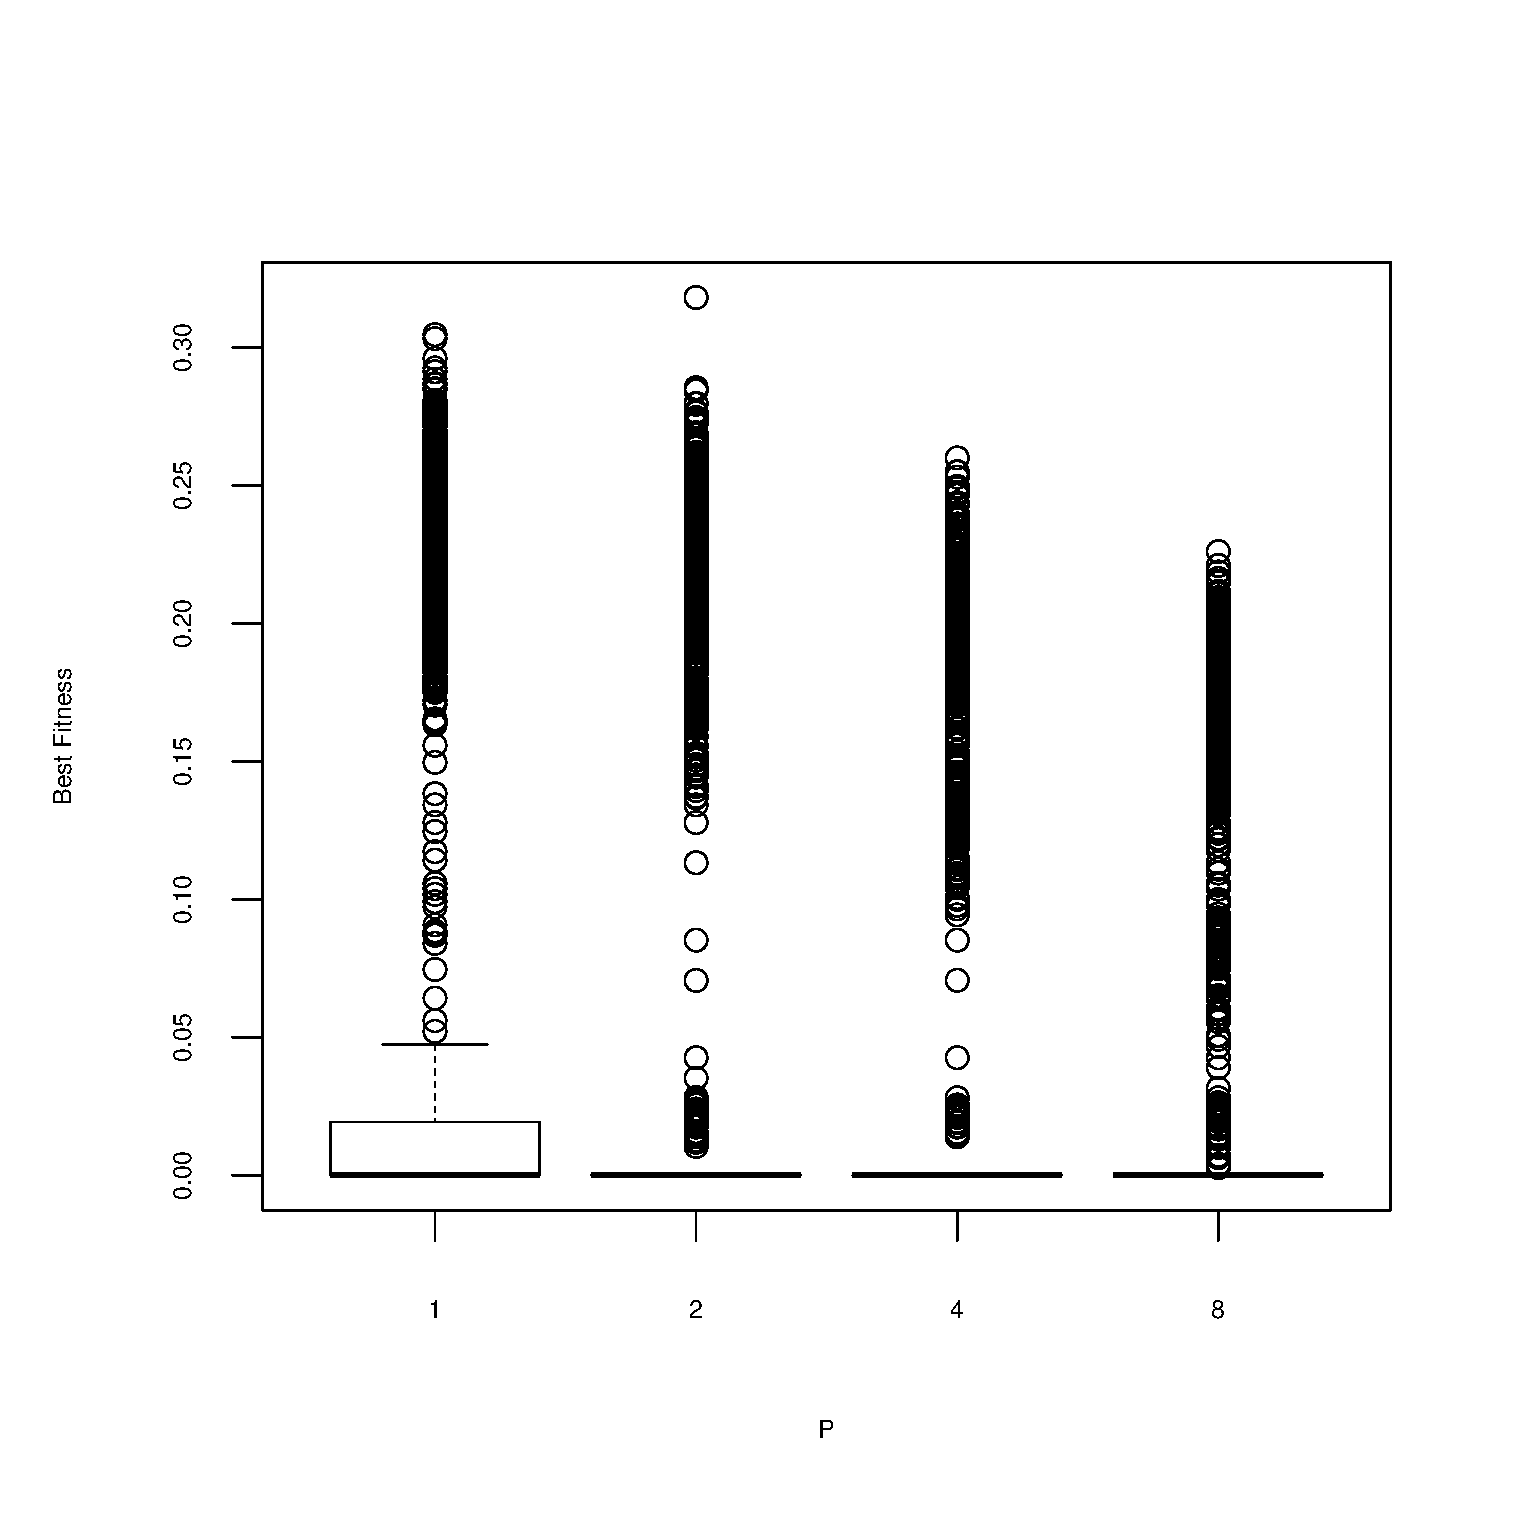
\includegraphics[width=3.7cm]{imags/boxplotz1P.eps}
                \label{fig:e1_p}
        }
        \subfigure[\scriptsize{Scenario 2: Hero}]{
                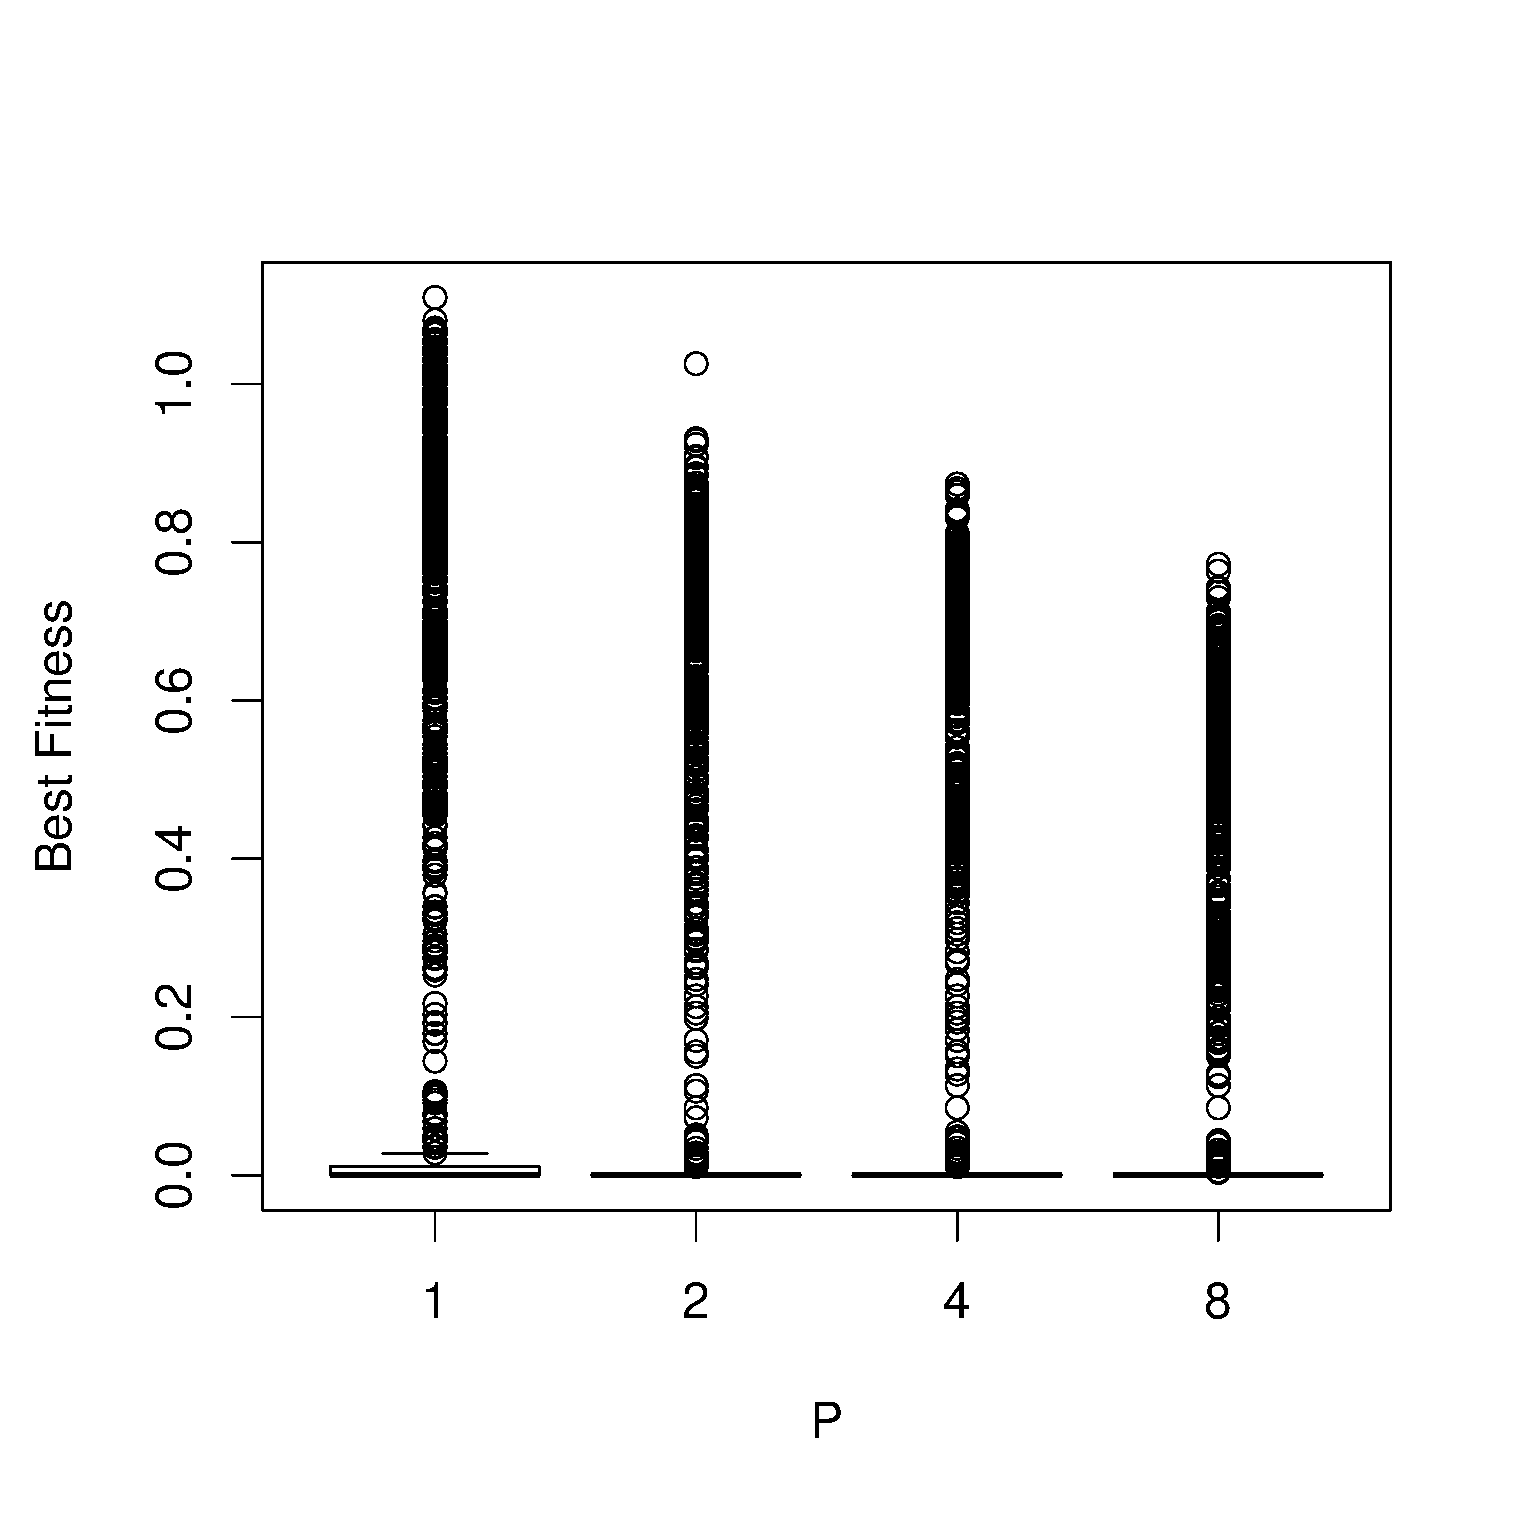
\includegraphics[width=3.7cm]{imags/boxplotz2P.eps}
                \label{fig:e2_p}
        }
        \subfigure[\scriptsize{Scenario 3: Avenger}]{
                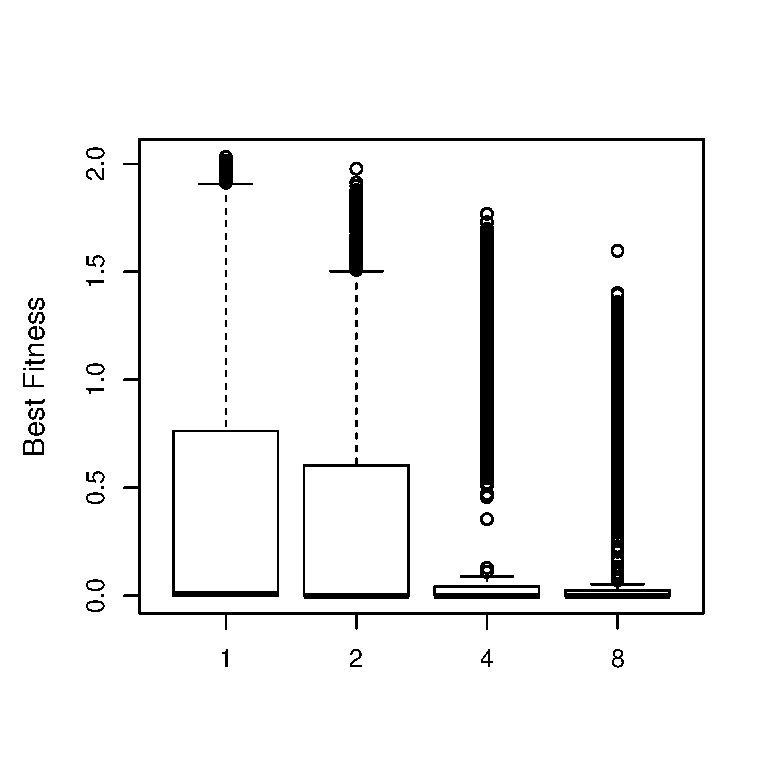
\includegraphics[width=3.7cm]{imags/boxplotz5P.eps}
                \label{fig:e3_p}
        }  
        \caption{Boxplots for parameter P (number of profiles)}\label{fig:boxplotsP}
\end{figure}
%
All the results have also been plotted in order to better understand 
their differences (in Figures \ref{fig:boxplotsP} to \ref{fig:boxplotsS}). At first glance, the median for D, W and F is 0 (or almost 0) for several
values. This has several possible explanations: First, the
number of profiles has quite an impact in the results (Figure
\ref{fig:boxplotsP}), as it was shown previously in
\cite{garcia:anon}. 

Increasing the number of profiles means changing the search problem
from finding a single finite state automaton whose behaviour
eventually results in a world compatible with our search to finding
two or more compatible with it and among themselves. This also happens
independently of the situation and including complex ones, like the
Avenger scenario, so for the time being we should conclude that a
single profile, that is, having the description of a single FSM that
describes the behavior of the agents in the world, is the best option for any scenario. 

\begin{figure}[h!tb]
        \centering
        \subfigure[\scriptsize{Scenario 1: Villain}]{
                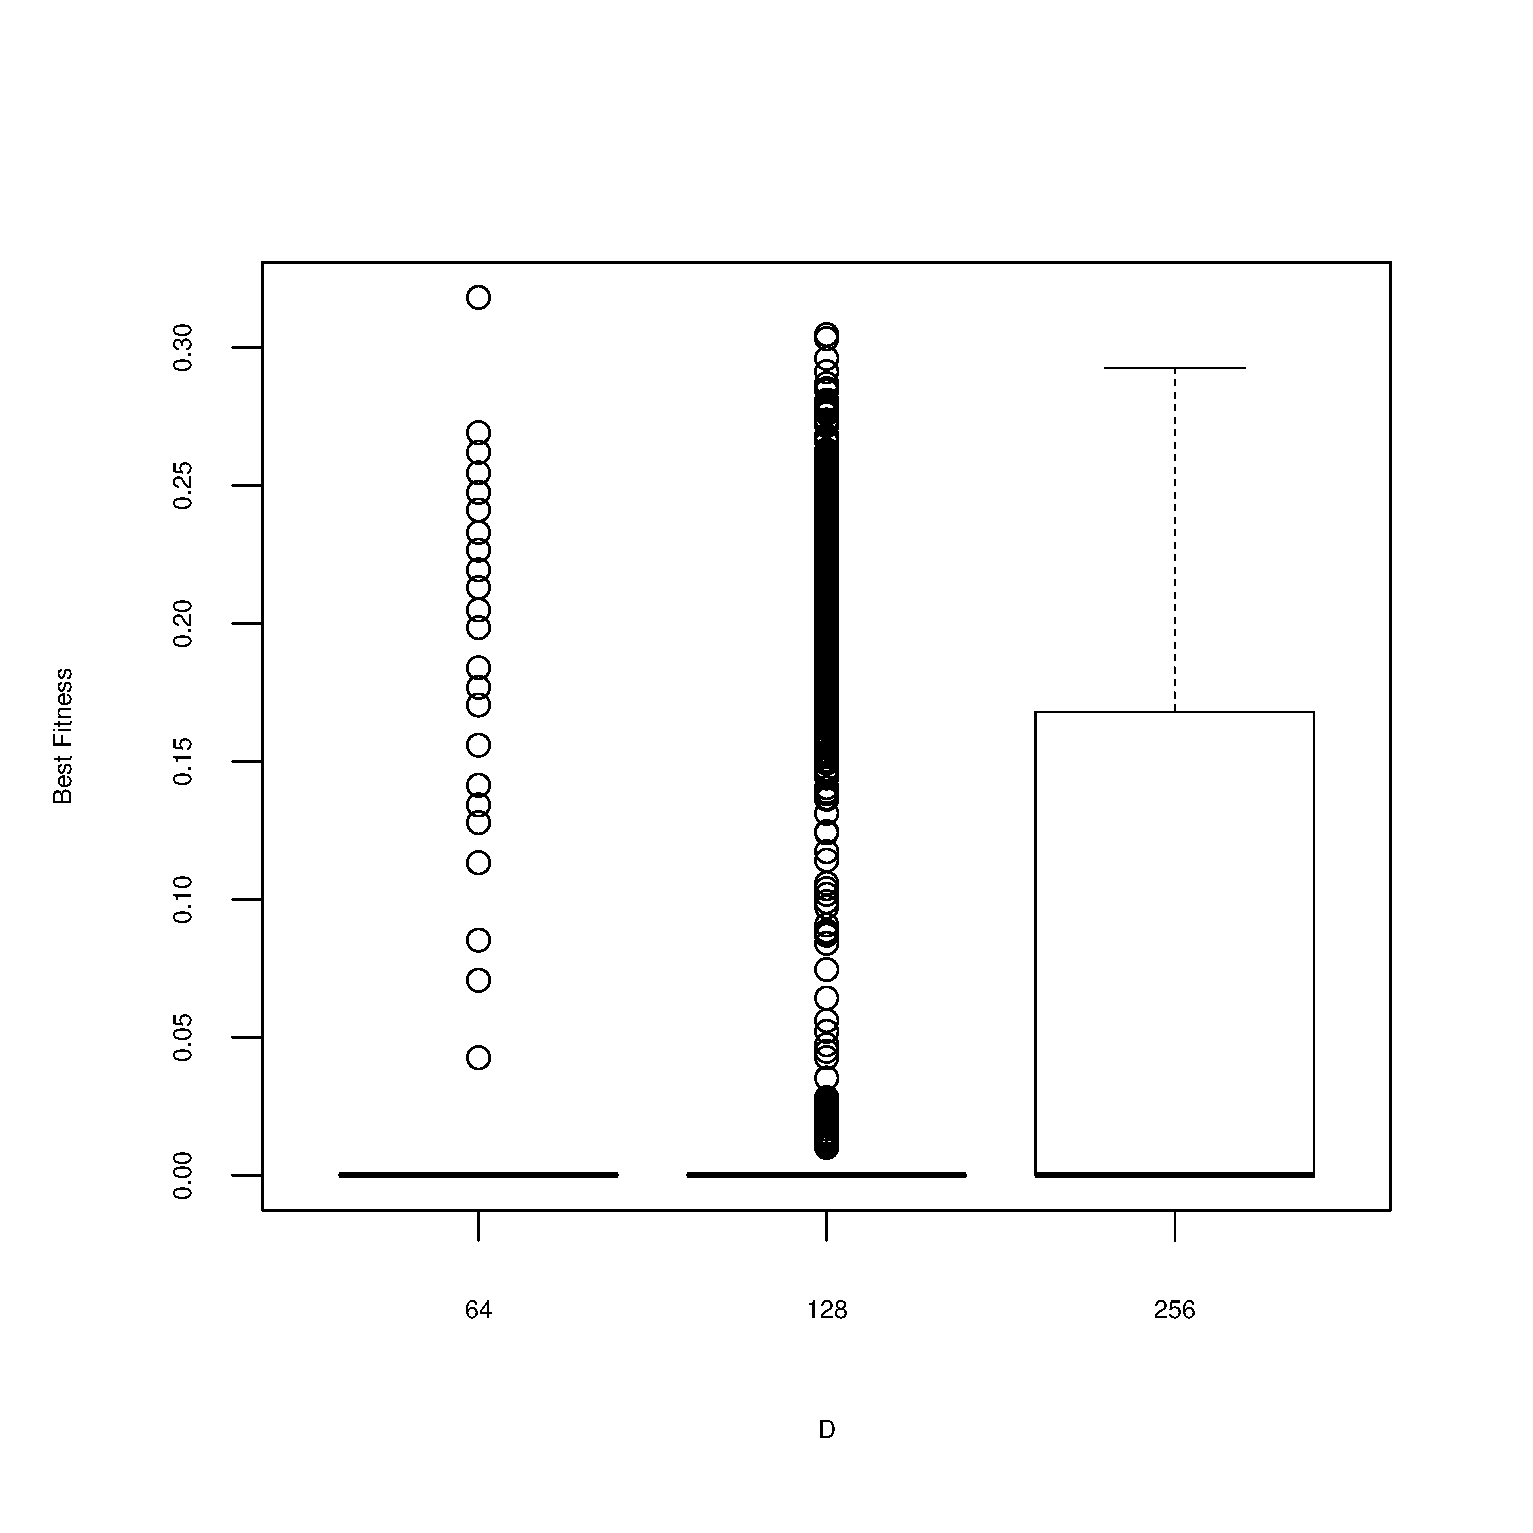
\includegraphics[width=3.7cm]{imags/boxplotz1D.eps}
                \label{fig:e1_d}
        }
        \subfigure[\scriptsize{Scenario 2: Hero}]{
                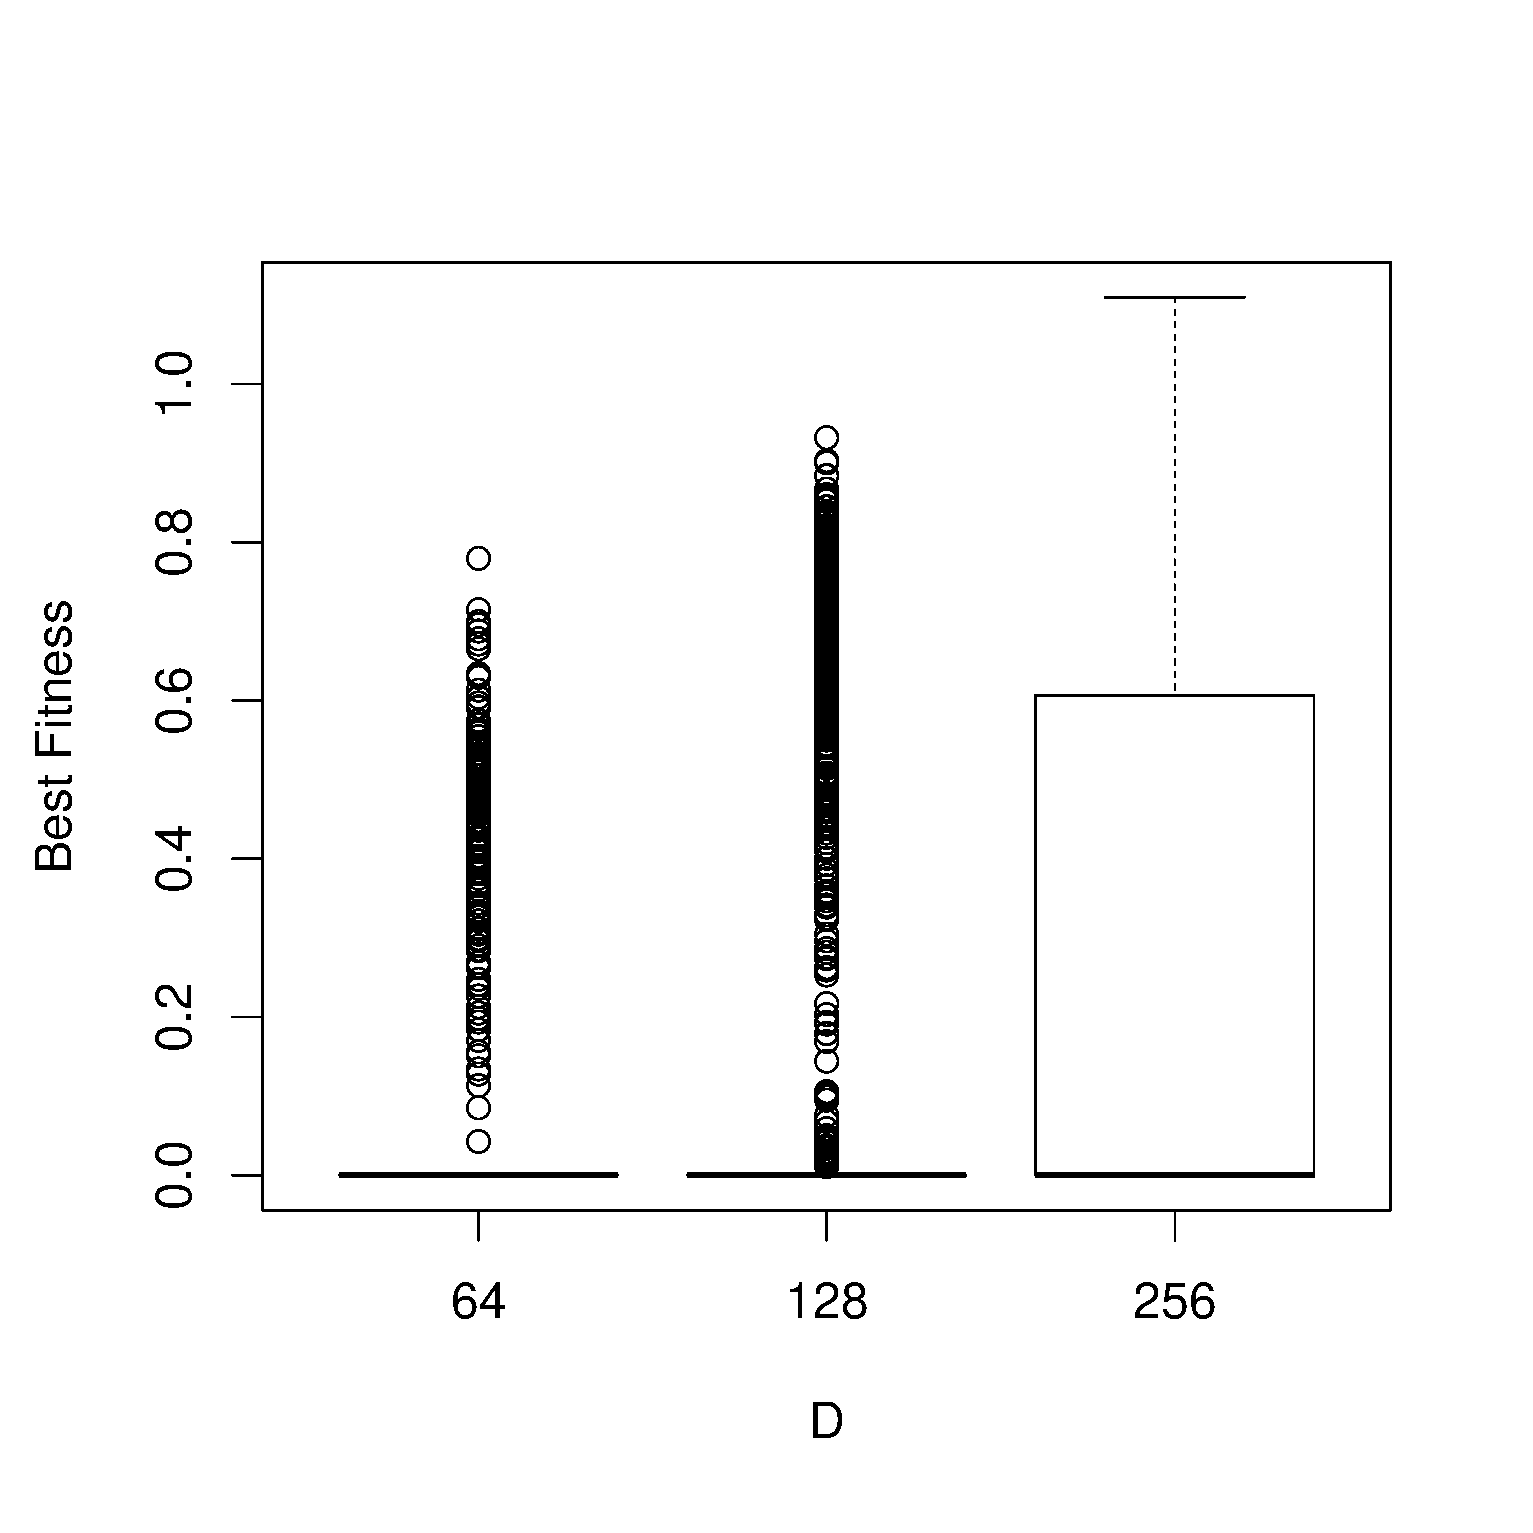
\includegraphics[width=3.7cm]{imags/boxplotz2D.eps}
                \label{fig:e2_d}
        }
        \subfigure[\scriptsize{Scenario 3: Avenger}]{
                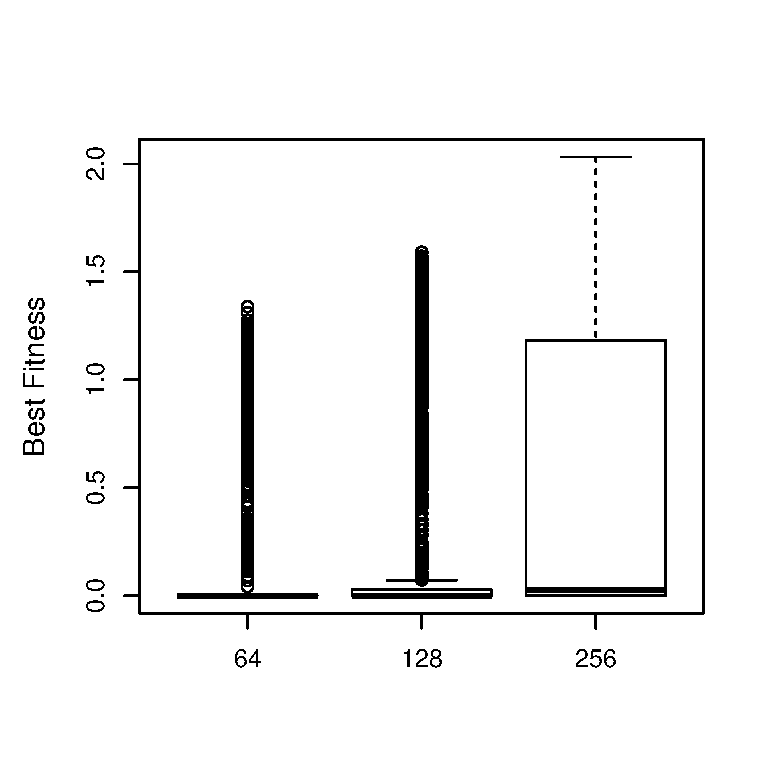
\includegraphics[width=3.7cm]{imags/boxplotz5D.eps}
                \label{fig:e3_d}
        }  
        \caption{Boxplots for the number of days (parameter D).}\label{fig:boxplotsD} 
\end{figure}

\begin{figure}[h!tb]
        \centering
        \subfigure[\scriptsize{Scenario 1: Villain}]{
                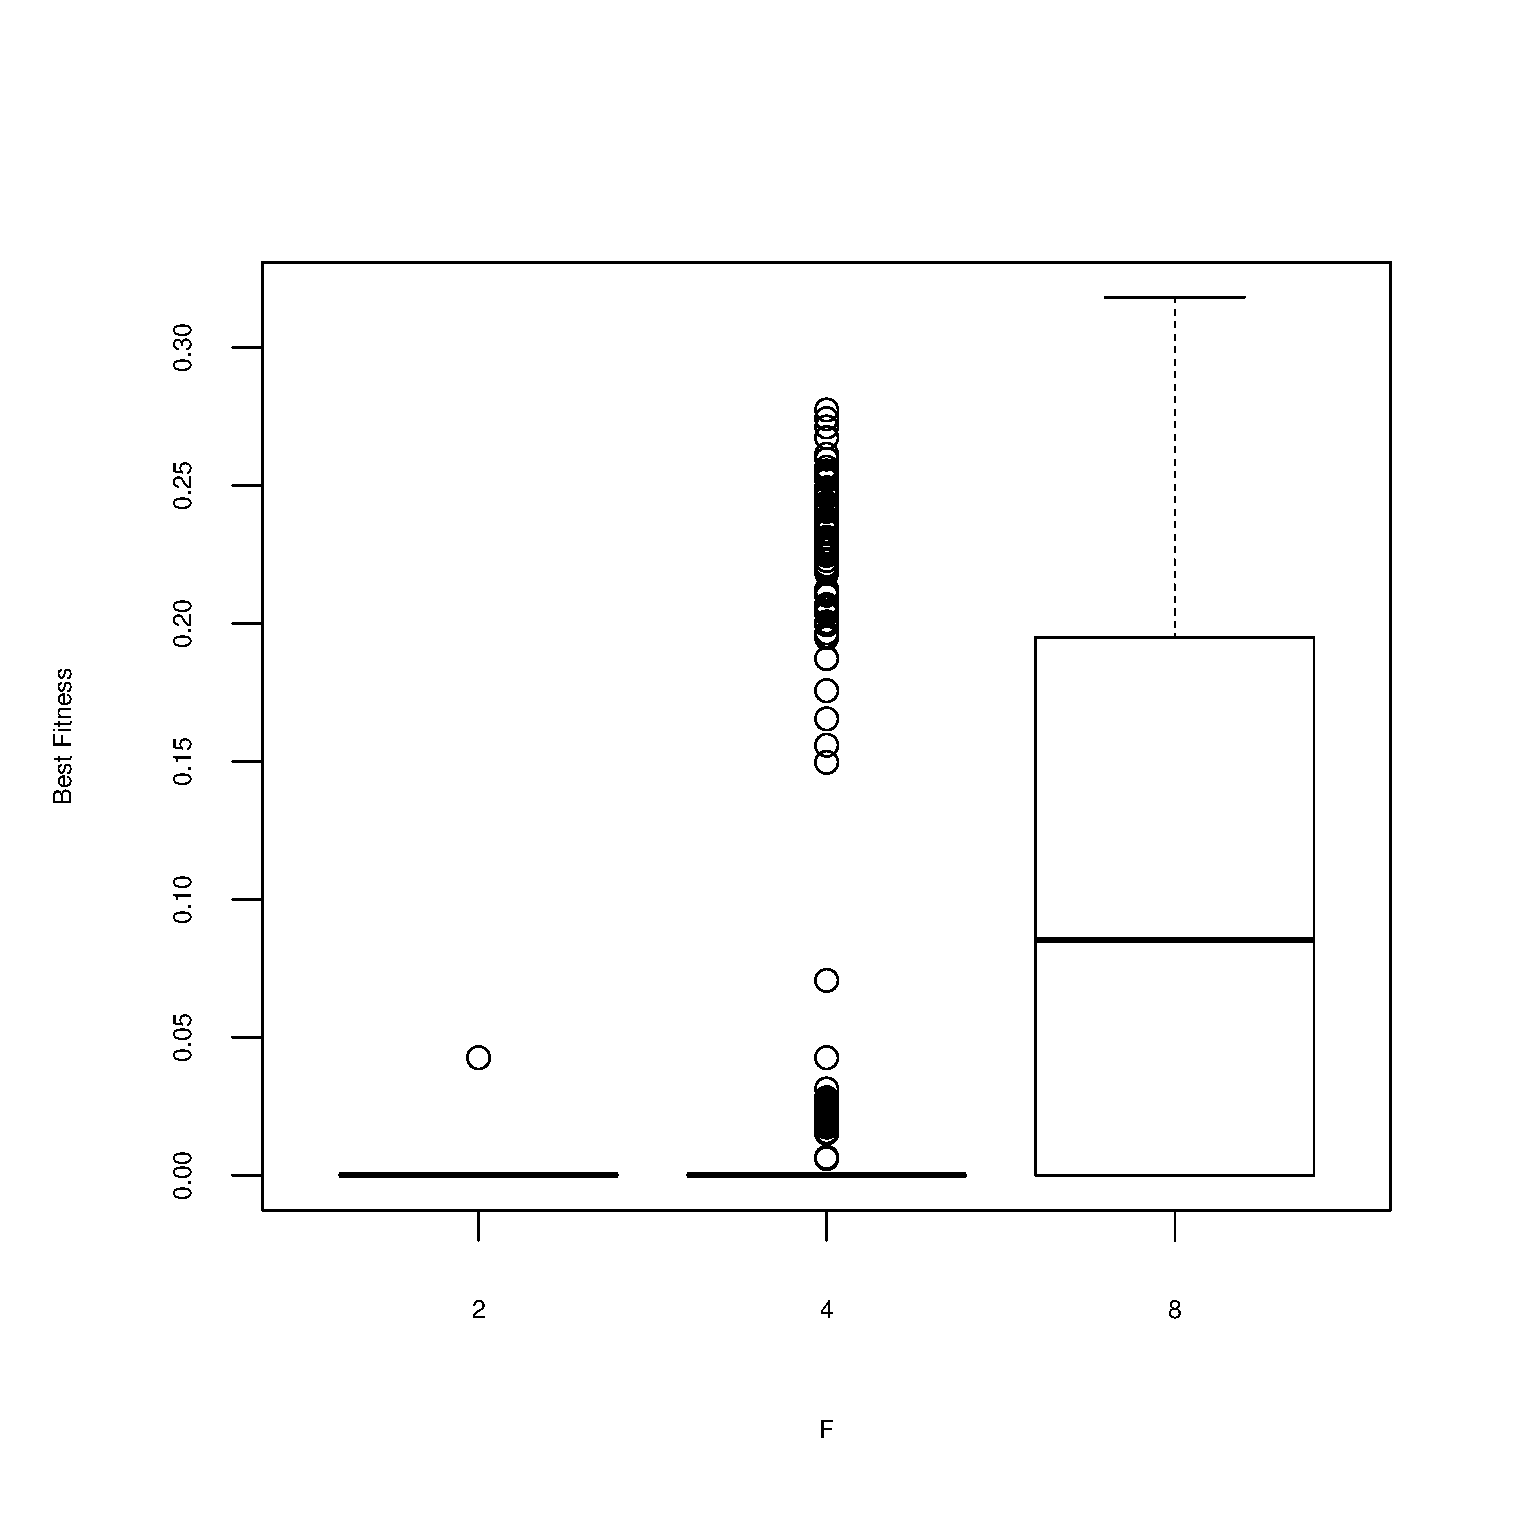
\includegraphics[width=3.7cm]{imags/boxplotz1F.eps}
                \label{fig:e1_f}
        }
        \subfigure[\scriptsize{Scenario 2: Hero}]{
                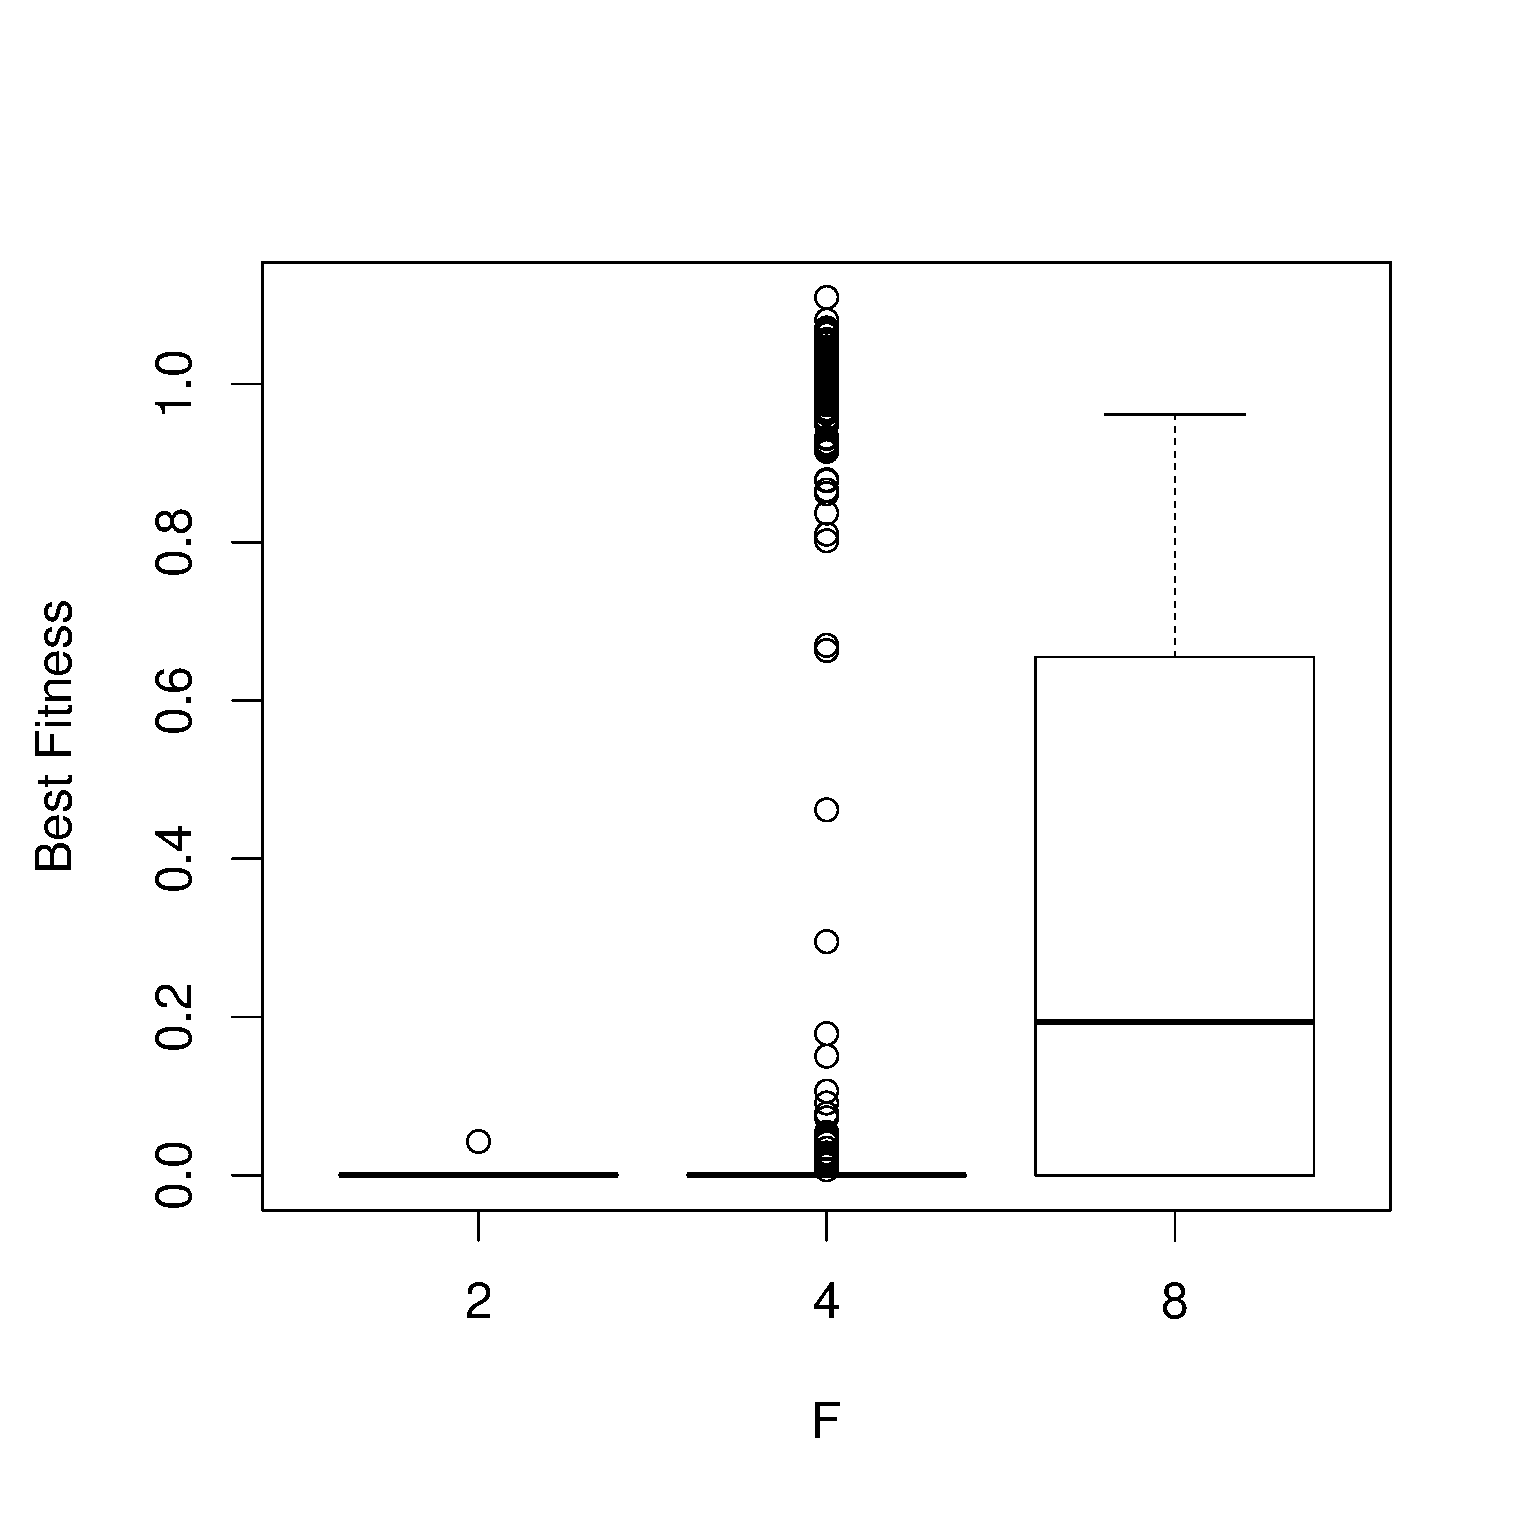
\includegraphics[width=3.7cm]{imags/boxplotz2F.eps}
                \label{fig:e2_f}
        }
        \subfigure[\scriptsize{Scenario 3: Avenger}]{
                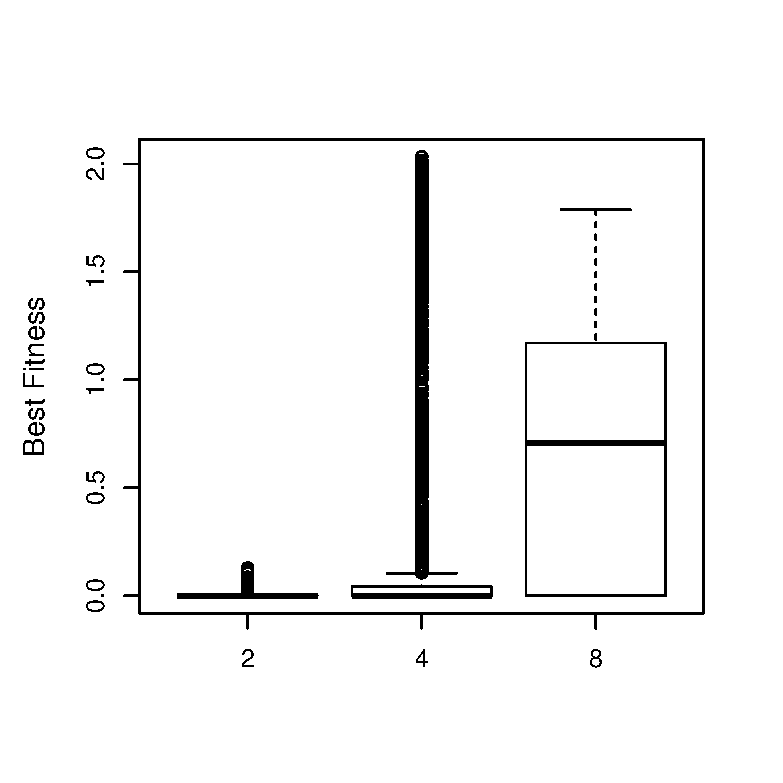
\includegraphics[width=3.7cm]{imags/boxplotz5F.eps}
                \label{fig:e3_f}
        }  
        \caption{Boxplots for food amount (parameter F)}\label{fig:boxplotsF}
\end{figure}

A similar result is obtained for the number of days, whose results in
the three scenarios can be seen in Figure \ref{fig:boxplotsD}: A small
amount of days (64) is not enough to allow the generation of any
archetype, as there is no time to develop a story, or, in another
words, for the events that we examine to compute fitness to occur, in
most of the scenarios. This can also be said
%
\begin{figure}[h!tb]
        \centering
        \subfigure[\scriptsize{Scenario 1: Villain}]{
                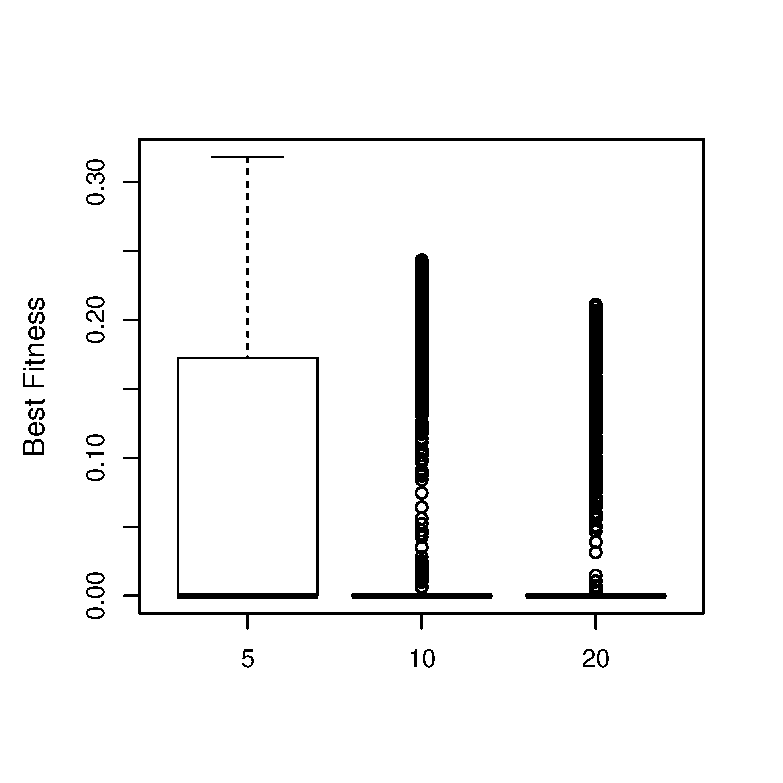
\includegraphics[width=3.7cm]{imags/boxplotz1W.eps}
                \label{fig:e1_w}
        }
        \subfigure[\scriptsize{Scenario 2: Hero}]{
                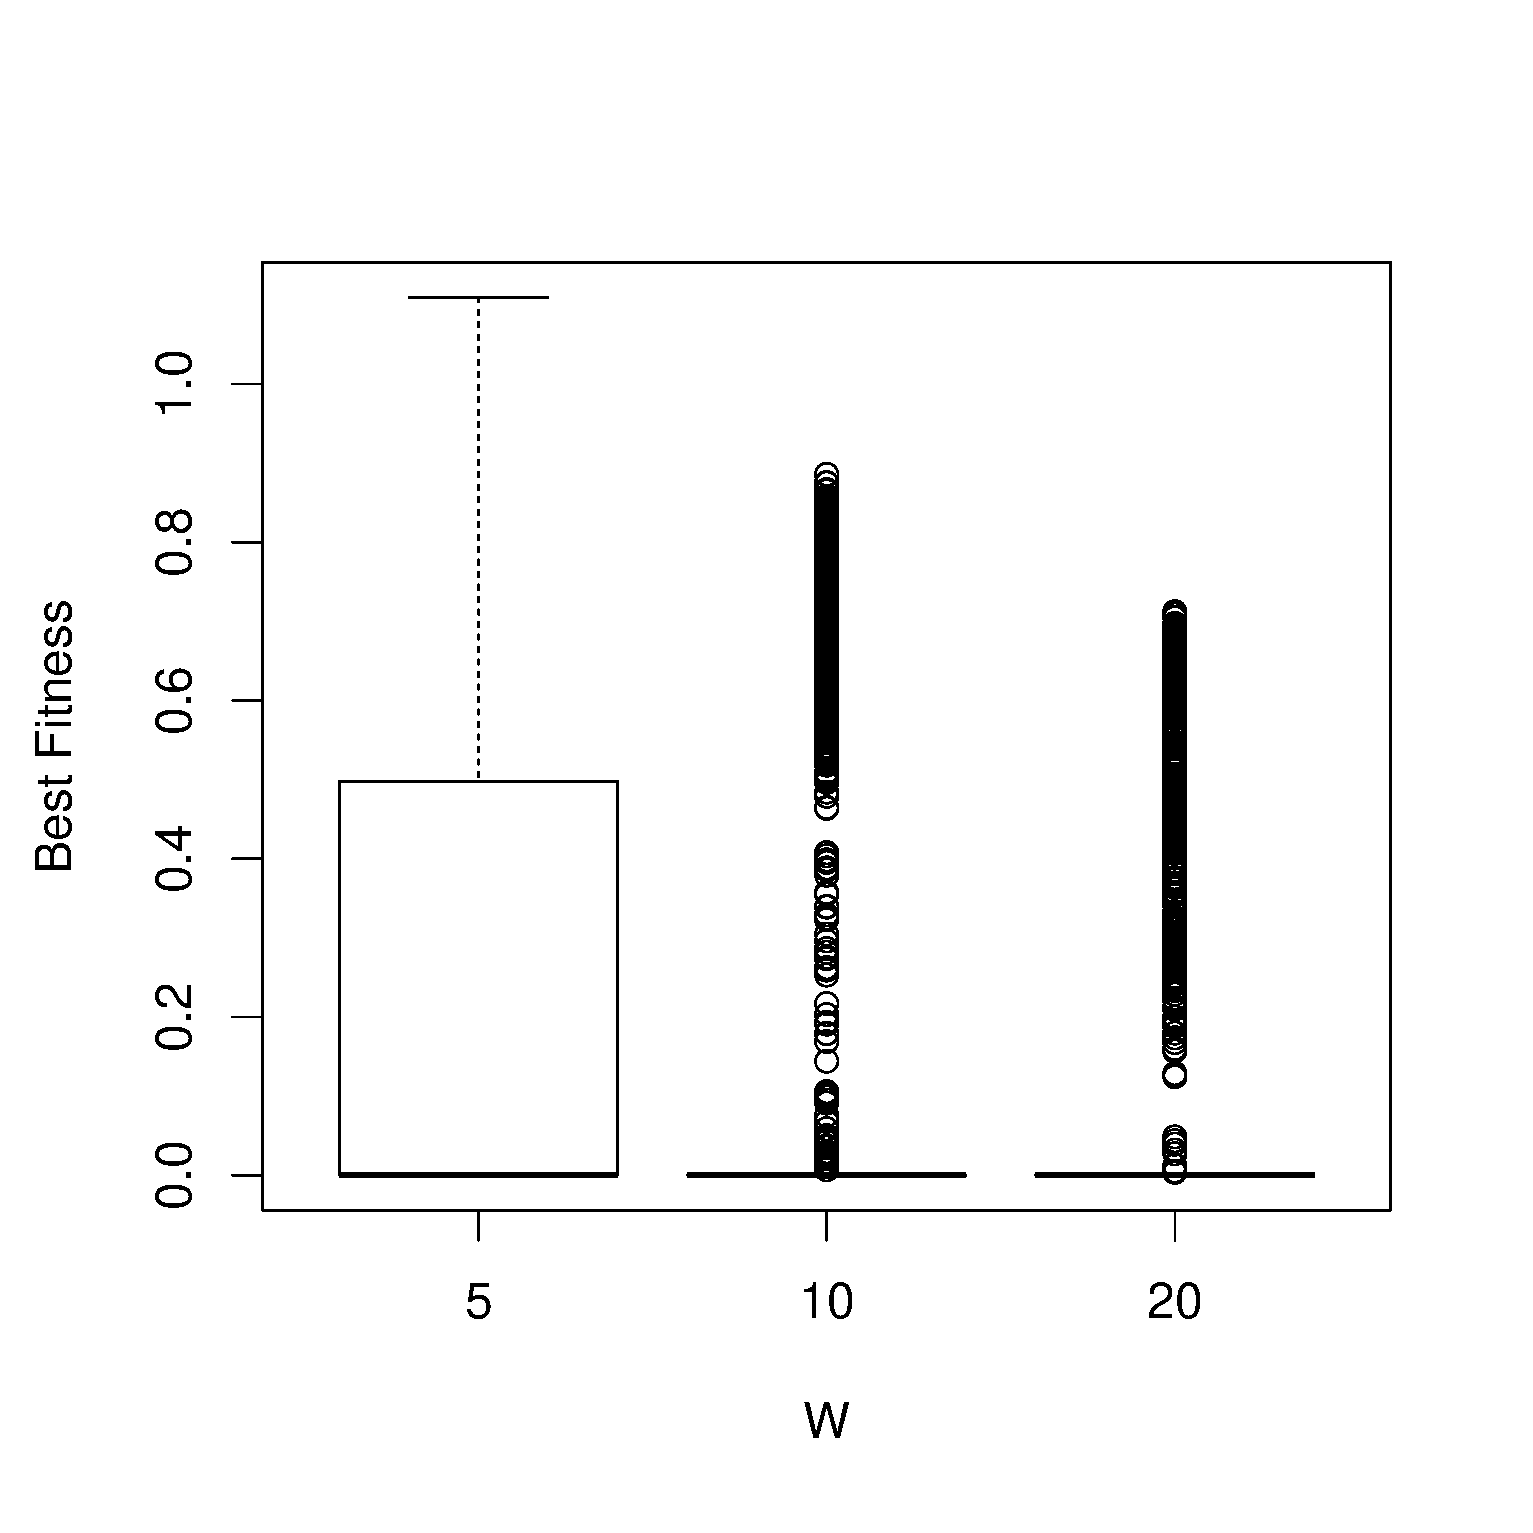
\includegraphics[width=3.7cm]{imags/boxplotz2W.eps}
                \label{fig:e2_w}
        }
        \subfigure[\scriptsize{Scenario 3: Avenger}]{
                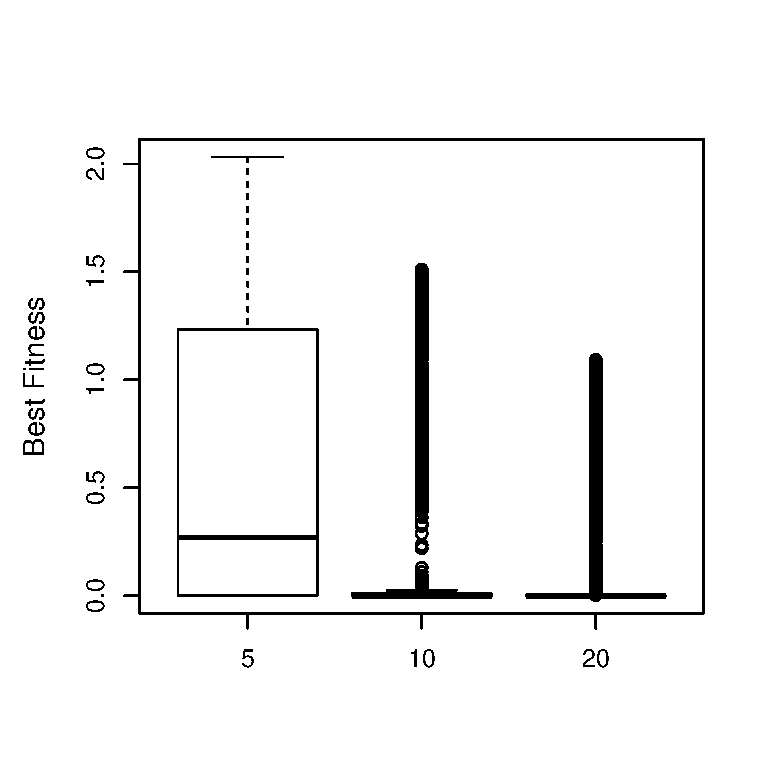
\includegraphics[width=3.7cm]{imags/boxplotz5W.eps}
                \label{fig:e3_w}
        }  
        \caption{Boxplots for world size (parameter W)}\label{fig:boxplotsW}
\end{figure}
%
about the world dimension (Figure \ref{fig:boxplotsW}): larger worlds
are more sparsely populated and have less interaction events, so the chances of an encounter that can trig an event (for
example, a fight) is more difficult. 

From the study of these two parameters we can conclude that, at least
for these scenarios and possibly for any scenario, the baseline number
of days should be 256 and the world for this population should have a
small size of 25 cells. 

\begin{figure}
        \centering
        \subfigure[\scriptsize{Scenario 1: Villain}]{
                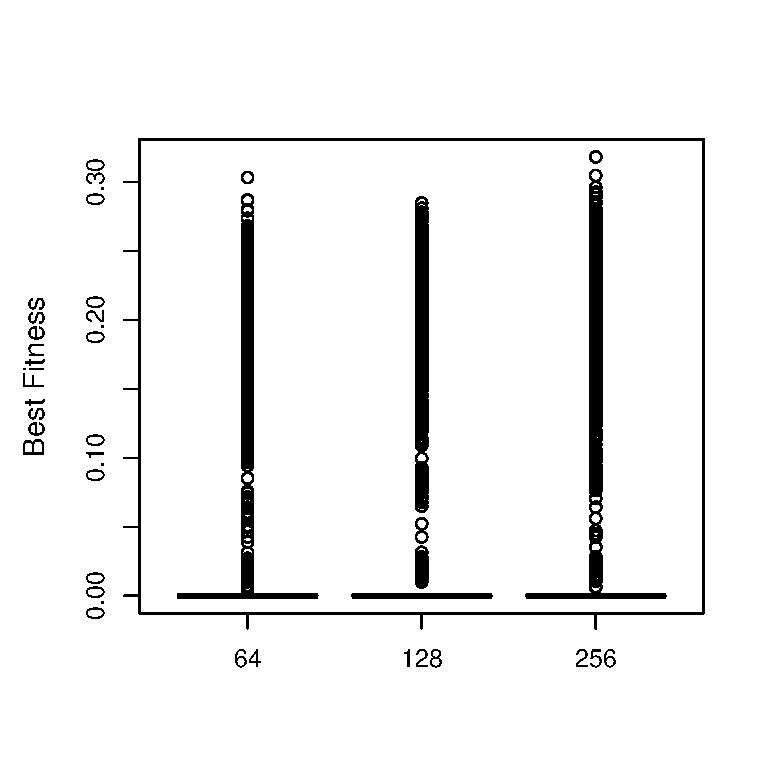
\includegraphics[width=3.7cm]{imags/boxplotz1S.eps}
                \label{fig:e1_s}
        }
        \subfigure[\scriptsize{Scenario 2: Hero}]{
                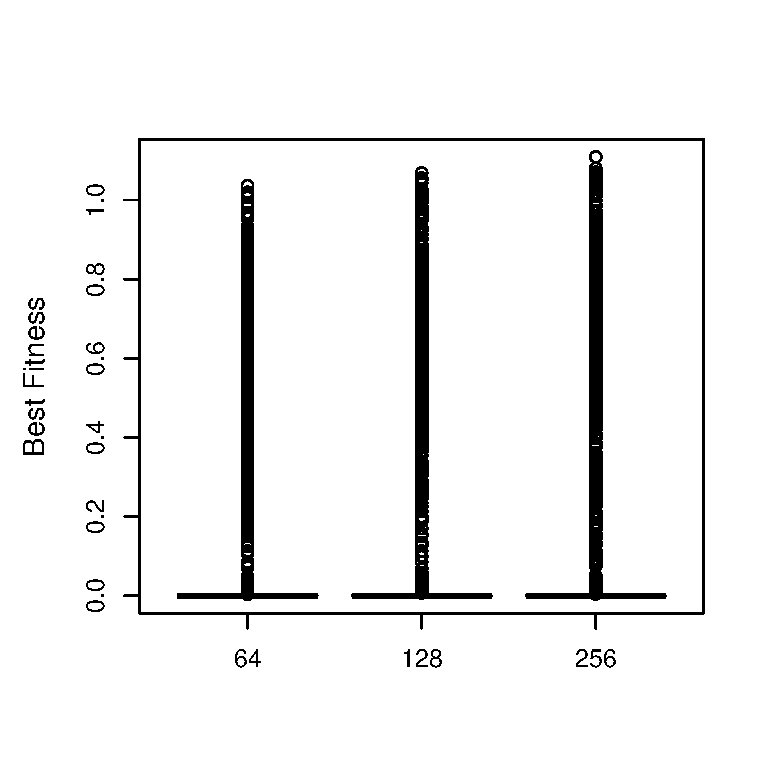
\includegraphics[width=3.7cm]{imags/boxplotz2S.eps}
                \label{fig:e2_s}
        }
        \subfigure[\scriptsize{Scenario 3: Avenger}]{
                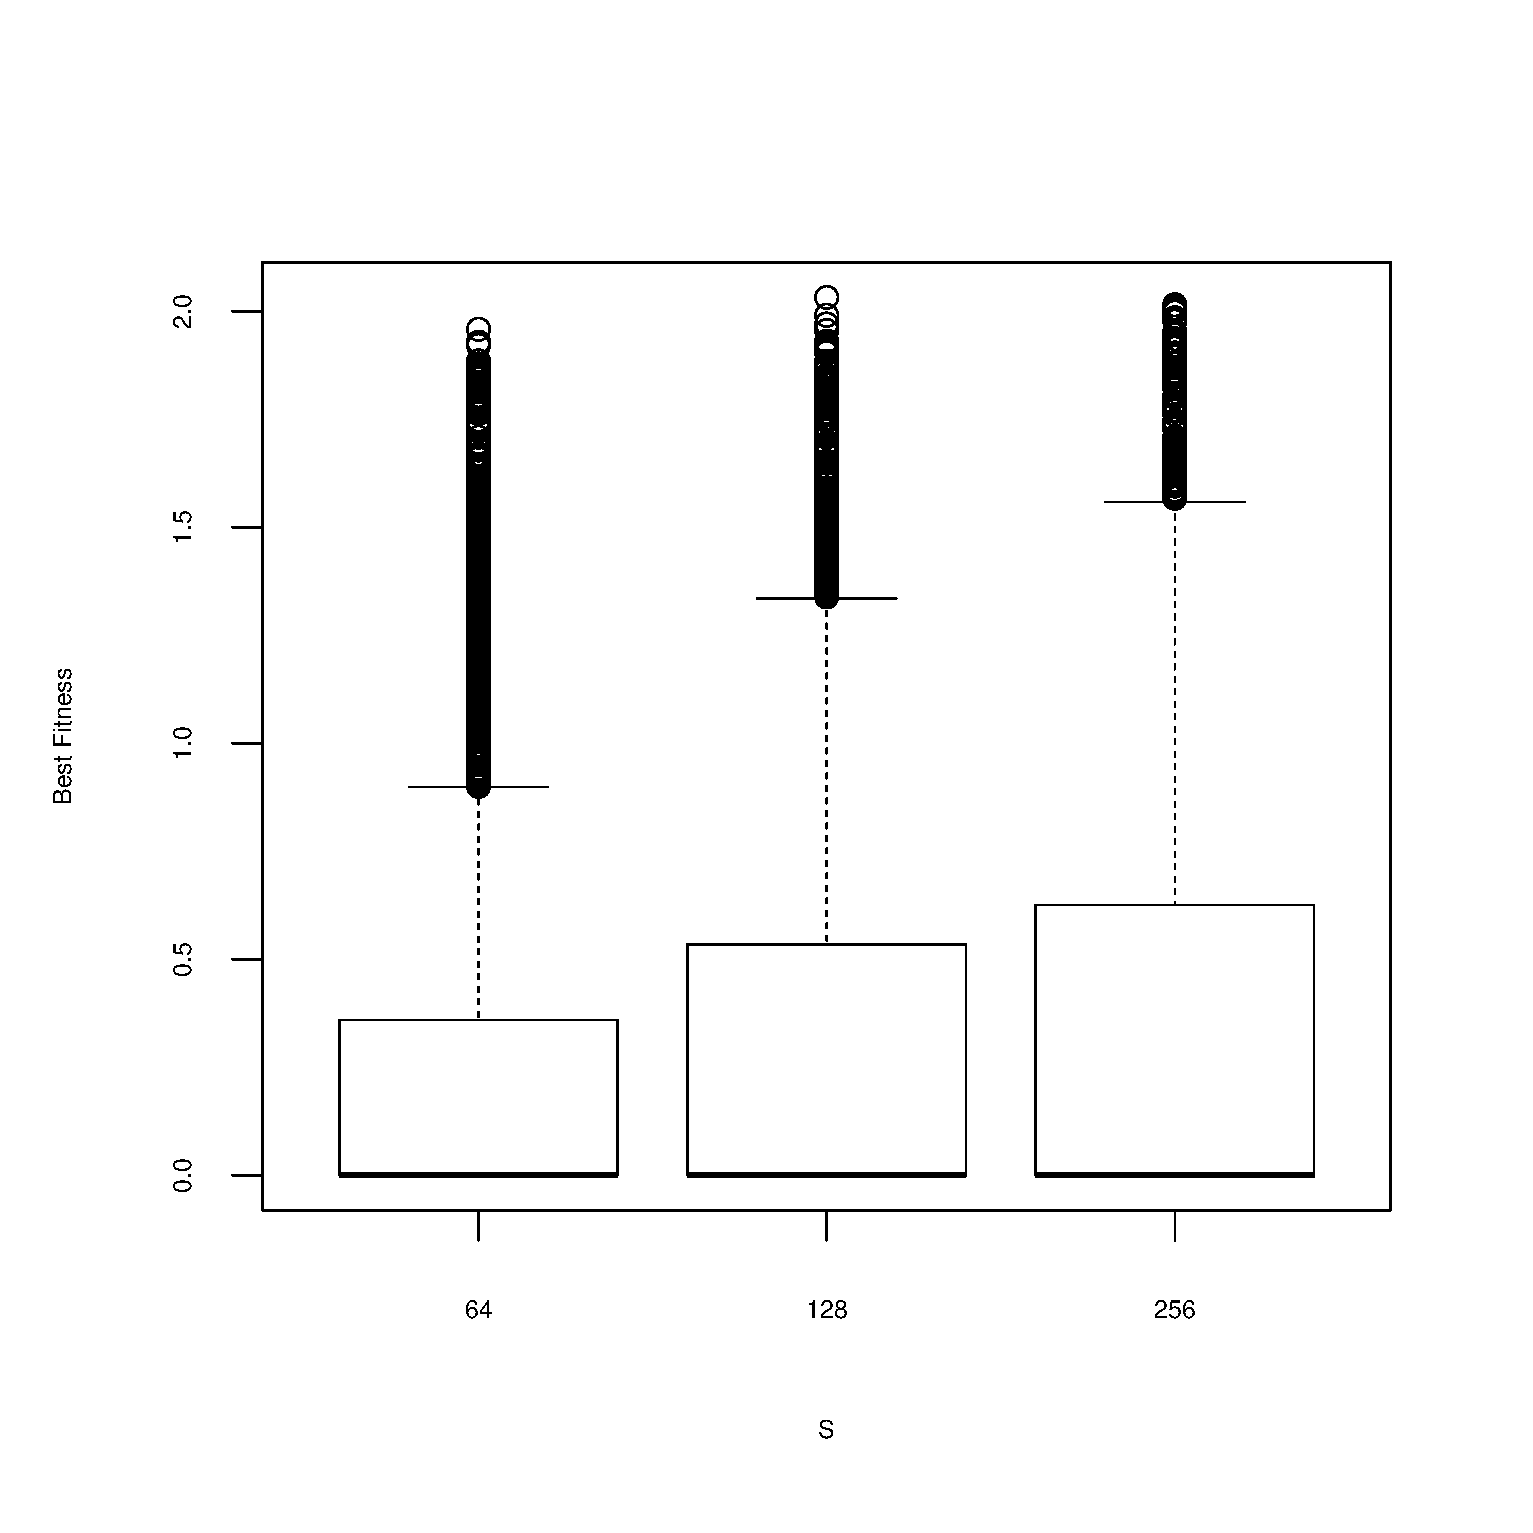
\includegraphics[width=3.7cm]{imags/boxplotz5S.eps}
                \label{fig:e3_s}
        }  
        \caption{Boxplots for GA population size (parameter S)}\label{fig:boxplotsS}
\end{figure}

Finally, the amount of food (Figure \ref{fig:boxplotsF}), which is 
the main source of conflicts, 
also needs to be low enough so that it actually happens, in this case 1/8
of the world size. 


With respect to the GA population size, Figure \ref{fig:boxplotsS} shows visually the confirmation of the tests: there are significant differences in the values for the Scenario 3. Because the large exploration space of this problem it is clear that larger sizes, in combination with a stop criterion based in changes of the best individual found, can obtain a higher range of possible solution values.


%%%%%%%%%%%%%%%%%%%%%%%%%%%%%%%%%%%%%%%%%%%%%%%%%%%%%%%%%%%%%%%%%%%%%%%%%%%%%%%
%%%%%%%%%%%%%%%%%%%%%%%%%%%%%%%%%%%%%%%%%%%%%%%%%%%%%%%%%%%%%%%%%%%%%%%%%%%%%%%


\section{Conclusions}

When using an hybrid EC-ABM approach to generate massive backstories in fiction environments its impossible to know in advance the
optimal value of a fitness that models the appearance of different archetypes
together and the search space may be enormous, so a previous study of
the most important parameters is prescribed. 

In this paper we define the problem addressed (in terms of goal,
worlds, fitnesses, archetypes, backstories, agents, profiles,
conflicts, places, time and scenario) and a problem specification with
the MADE framework. Our methodology selects key parameters (size of
population of the GA, size of the world, number of profiles, source of
conflicts and virtual days) that affect the generation of conflicts
and sets the values that are tested in the experiments, looking for
significant differences in the fitness of the evolved worlds. 

Our experiments prove that there are significant differences between
the five parameters in three scenarios with different combinations of
the archetype \textit{villain}, \textit{hero} and
\textit{avenger}. The best combination of parameters, that is, the one
that gives on average the highest fitness, is the smallest map size
(5x5), the bigger number of virtual days (256), the fewer rate of food
growth (1/8 of the number of cells), the lower number of profiles (1)
and the bigger population size of the GA (256). This is due to the
fact that the three possible archetypes emerge when a the fights
occur, and that happens more probably when the world is small and
there is little food. Anyway, the backstories size increase with the
virtual days of execution, thus it is easier to find archetypes when
more virtual days are executed, in other words, when all the agents have
the opportunity to live their entire lives.
This can be generalised to similar problems (and the
rest of scenarios): the source of conflict should be forced to occur
more times, and simultaneously, it is necessary to give enough time to
these situations appear. 

%FERGU: Este p�rrafo que sigue no tiene ni pies ni cabeza, fuera :/
%This points to the fact that the number of virtual days might not be
%an adequate termination condition for the world, since what we are
%looking for is a series of facts to occur so that {\em
%  interesting} stories and relationships are generated. Using those
%facts (maybe combined with a maximum amount of days) might be a better
%termination condition for the world.

Another conclusion is that, even if the number of profiles (different
behaviours in the world) could, a priori, allow for more complex
archetypes to appear, the fact that they are codified in a chromosome
changes the shape of the search space and increases its size and
complexity, so that the number of generations the algorithm needs
might be much more. It is never easy to establish termination
conditions in these kind of evolutionary algorithms, so this is
something that should be researched in the future.

Since it has been proved that conflicts, as in fiction, is what drives
fitness up in the worlds we are designing, the actual number of conflicts happening in the world, its
influence in the fitness and its relationship with world size and food
growth will have to be assessed in future works. The influence of
parameters such as the initial population could be tested, while different scenarios will be used
with archetypes that not only rely in competition for food, like the
affinity or the family relationships. To improve the accuracy of the
parameter selection, human guided evaluation could be
performed, but this is only one possible way of doing it. Finally, the
results of the study could be applied to 
generate backstories in real game engines. 

\section*{Acknowledgements}

Hidden for double-blind review

\bibliographystyle{splncs03}
\bibliography{geneura,references}

\end{document}
